\documentclass[11pt]{amsart}
\usepackage{geometry}                % See geometry.pdf to learn the layout options. There are lots.
\geometry{letterpaper}                   % ... or a4paper or a5paper or ... 
%\geometry{landscape}                % Activate for for rotated page geometry
%\usepackage[parfill]{parskip}    % Activate to begin paragraphs with an empty line rather than an indent
\usepackage{graphicx}
\usepackage{amssymb}
\usepackage{float}
\usepackage{python}
\usepackage{epstopdf}
\usepackage{listings}
\usepackage{color}
 
\definecolor{codegreen}{rgb}{0,0.6,0}
\definecolor{codegray}{rgb}{0.5,0.5,0.5}
\definecolor{codepurple}{rgb}{0.58,0,0.82}
\definecolor{backcolour}{rgb}{0.95,0.95,0.92}
 
\lstdefinestyle{mystyle}{
    %backgroundcolor=\color{backcolour},   
    commentstyle=\color{codegreen},
    keywordstyle=\color{magenta},
    numberstyle=\tiny\color{codegray},
    stringstyle=\color{codepurple},
    basicstyle=\footnotesize,
    breakatwhitespace=false,         
    breaklines=true,                 
    captionpos=b,                    
    keepspaces=true,                 
    numbers=left,                    
    numbersep=5pt,                  
    showspaces=false,                
    showstringspaces=false,
    showtabs=false,                  
    tabsize=2
}
 
\lstset{style=mystyle}
\DeclareGraphicsRule{.tif}{png}{.png}{`convert #1 `dirname #1`/`basename #1 .tif`.png}

\title{Homework 7}
\author{Carter Rhea}
\date{\today}                                           

\begin{document}
\maketitle
\section{Problem 1}
Statement: Show that the Q8 element does not present the problem of shear locking.
Proceed in the same manner as was shown for the Q4 element in class. That is, use the
given continuous displacement field to compute displacements at nodes, calculate strains
in the element using the element interpolation functions, and then compare these to the
exact solution.
\\
Solution: \\
From class we know: $$U_x = xcy $$
$$U_y = \frac{-cx^2}{2} $$
$$\mathcal{E}_{xx} = \frac{\partial U_x}{\partial x} = cy $$
$$\mathcal{E}_{yy} = \frac{\partial U_y}{\partial y} = 0 $$
$$\mathcal{E}_{xy} = \frac{1}{2}\Big[\frac{\partial U_x}{\partial x}+\frac{\partial U_y}{\partial y}\Big] $$
We shall define $U$ similarly as was done in class,
$$
U = 
  \begin{Bmatrix}
  1\\
  -1/2\\
  -1\\
  -1/2\\
  1\\
  -1/2\\
  -1\\
  -1/2\\
  0\\
  0\\
  0\\
  -1/2\\
  0\\
  0\\
  0\\
  -1/2\\
  \end{Bmatrix}
$$
The following is my Matlab code:
 \begin{lstlisting}[language=Matlab]
    x = sym('x'); y = sym('y'); c = sym('c');
    d = c*[1;-1/2;-1;-1/2;1;-1/2;-1;-1/2;0;0;0;-1/2;0;0;0;-1/2];
    N_1 = -(1/4)*(1-x)*(1-y)*(1+x+y);
    N_2 = -(1/4.)*(1+x)*(1-y)*(1-x+y);
    N_3 = -(1/4.)*(1+x)*(1+y)*(1-x-y);
    N_4 = -(1/4.)*(1-x)*(1+y)*(1+x-y);
    N_5 = (1/2.)*(1-x^2)*(1-y);
    N_6 = (1/2.)*(1+x)*(1-y^2);
    N_7 = (1/2.)*(1-x^2)*(1+y);
    N_8 = (1/2.)*(1-x)*(1-y^2);

%The following will create a vector of shape functions given a point
    N = zeros(2,16);
    N = sym('N');
    N(1,1) = N_1;
    N(1,3) = N_2;
    N(1,5) = N_3;
    N(1,7) = N_4;
    N(1,9) = N_5;
    N(1,11) = N_6;
    N(1,13) = N_7;
    N(1,15) = N_8;
    N(2,2) = N_1;
    N(2,4) = N_2;
    N(2,6) = N_3;
    N(2,8) = N_4;
    N(2,10) = N_5;
    N(2,12) = N_6;
    N(2,14) = N_7;
    N(2,16) = N_8;
    
    U = N*d;
    U = simplify(U);
    E_xx = diff(U(1),x);
    E_yy = diff(U(2),y);
    E_xy = 1./2*(diff(U(2),x)+diff(U(1),y));

\end{lstlisting}

This will yield 
$$U_x = c*x*y \ ;  \ U_y  = -(c*x^2)/2 $$
$$ \mathcal{E}_{xx} = c*y \  ; \  \mathcal{E}_{yy} = 0 \ ; \ \mathcal{E}_{xy} = 0$$

\section{Problem 2}
Complete the Matlab code provided with this homework and compute the
nodal displacements for the assembly of elements given below. You are given the main
script in a file called FEScript.m.

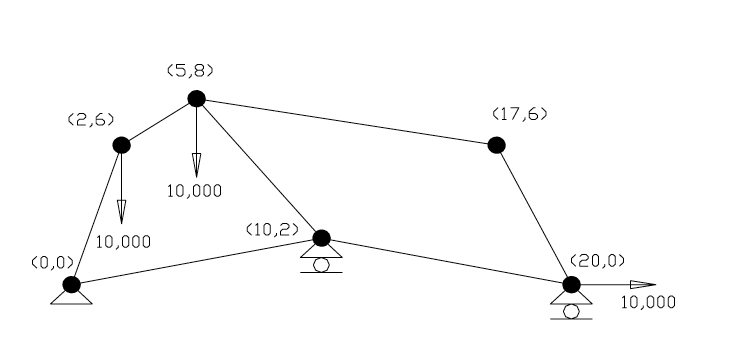
\includegraphics[scale=0.5]{P2_formulation.png}

I wont include my code here because that would be insane, but I will include an image showing the final displacement of the nodes

\begin{figure}
  \caption{The solid line is the undeformed mesh, the dashed line is the mesh deformed by my code, and the dotted line is the mesh deformed by ANSYS. }
  \centering
    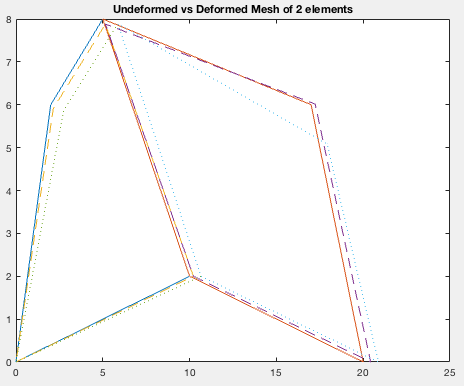
\includegraphics[width=0.5\textwidth]{P2.png}
\end{figure}
In the configuration in Problem 2, determine the eigenvalues and
eigenvectors of the stiffness matrix for these two cases.
\begin{enumerate}
	\item Full Integration
	\item Reduced Integration
\end{enumerate}
Plot the eigenvectors and report the number of zero eigenvalues in each case. Is the
number of zero eigenvalues as expected? Provide a brief justification to your answer.
\pagebreak[4] 



\section{Problem 3}
\subsection{Full Integration}
\subsection{Reduced Integration}


\begin{figure}[H] 
  \label{fig1} 
  \begin{minipage}[b]{0.5\linewidth}
    \centering
    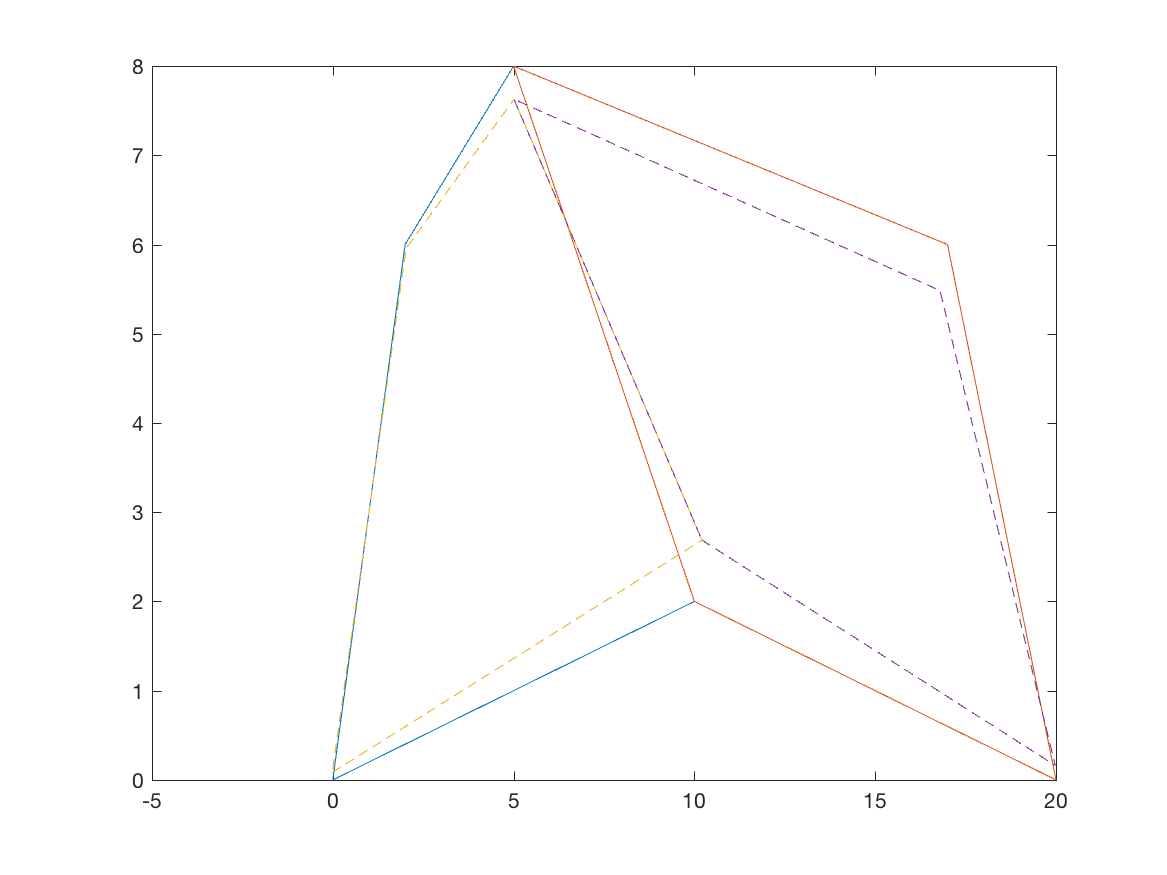
\includegraphics[width=.5\linewidth]{eigenvectors/eigenvector_1_fullint.png} 
    \caption{Eigenvalue 1} 
    \vspace{4ex}
  \end{minipage}%%
  \begin{minipage}[b]{0.5\linewidth}
    \centering
    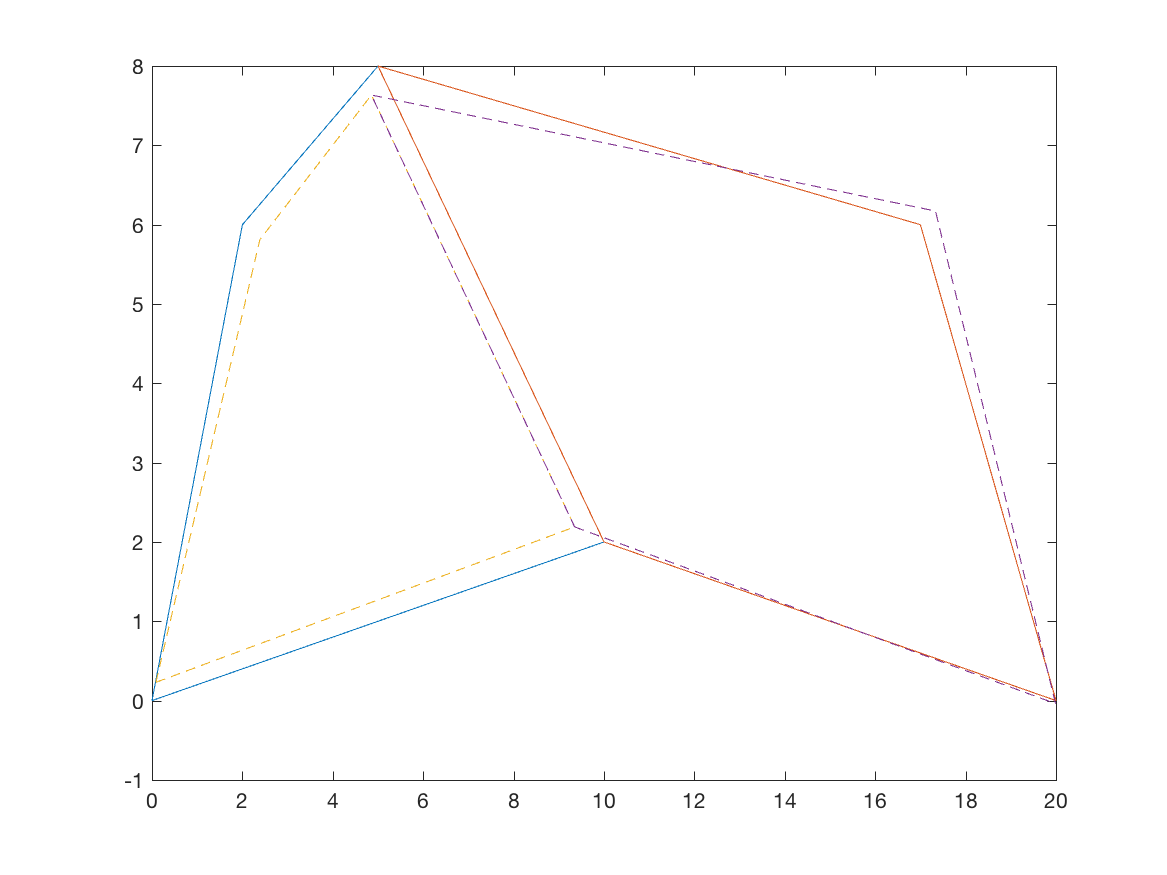
\includegraphics[width=.5\linewidth]{eigenvectors/eigenvector_2_fullint.png} 
    \caption{Eigenvalue 2} 
    \vspace{4ex}
  \end{minipage} 
  \begin{minipage}[b]{0.5\linewidth}
    \centering
    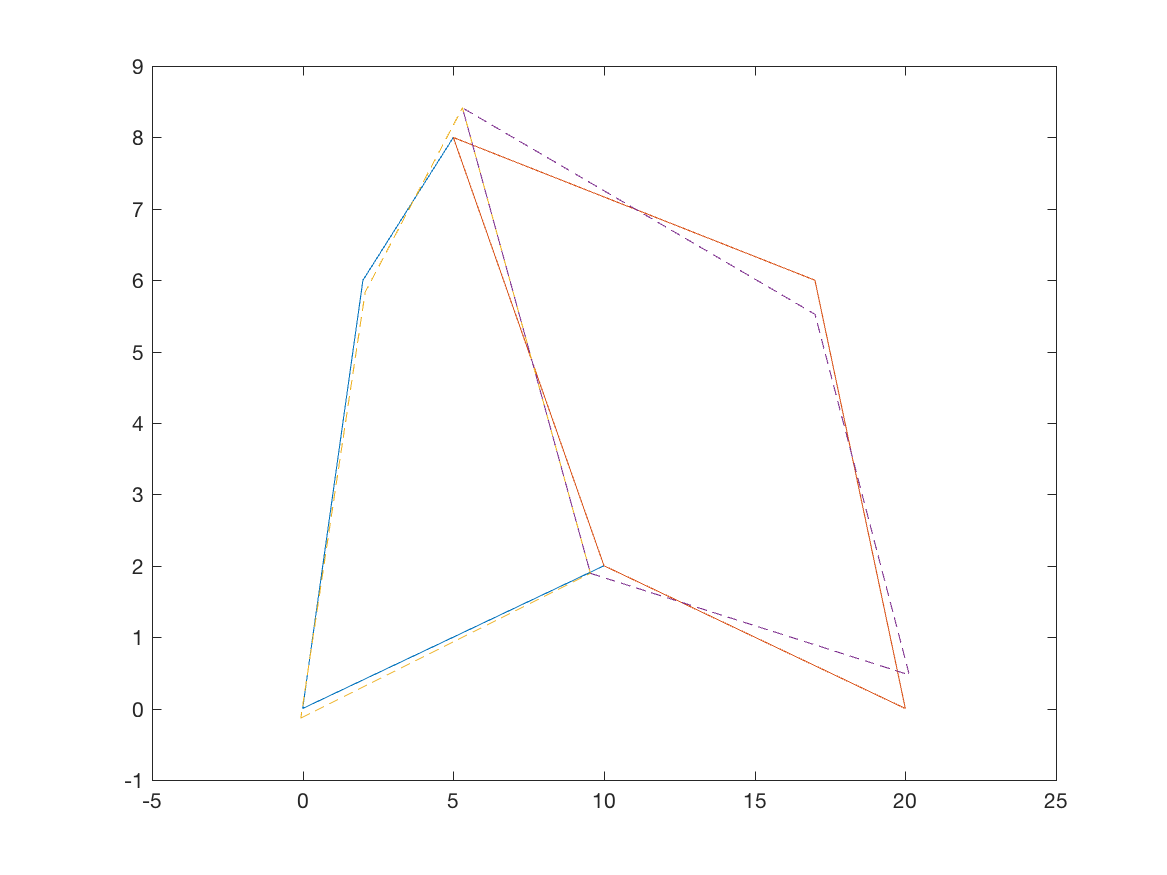
\includegraphics[width=.5\linewidth]{eigenvectors/eigenvector_3_fullint.png} 
    \caption{Eigenvalue 3} 
    \vspace{4ex}
  \end{minipage}%% 
  \begin{minipage}[b]{0.5\linewidth}
    \centering
    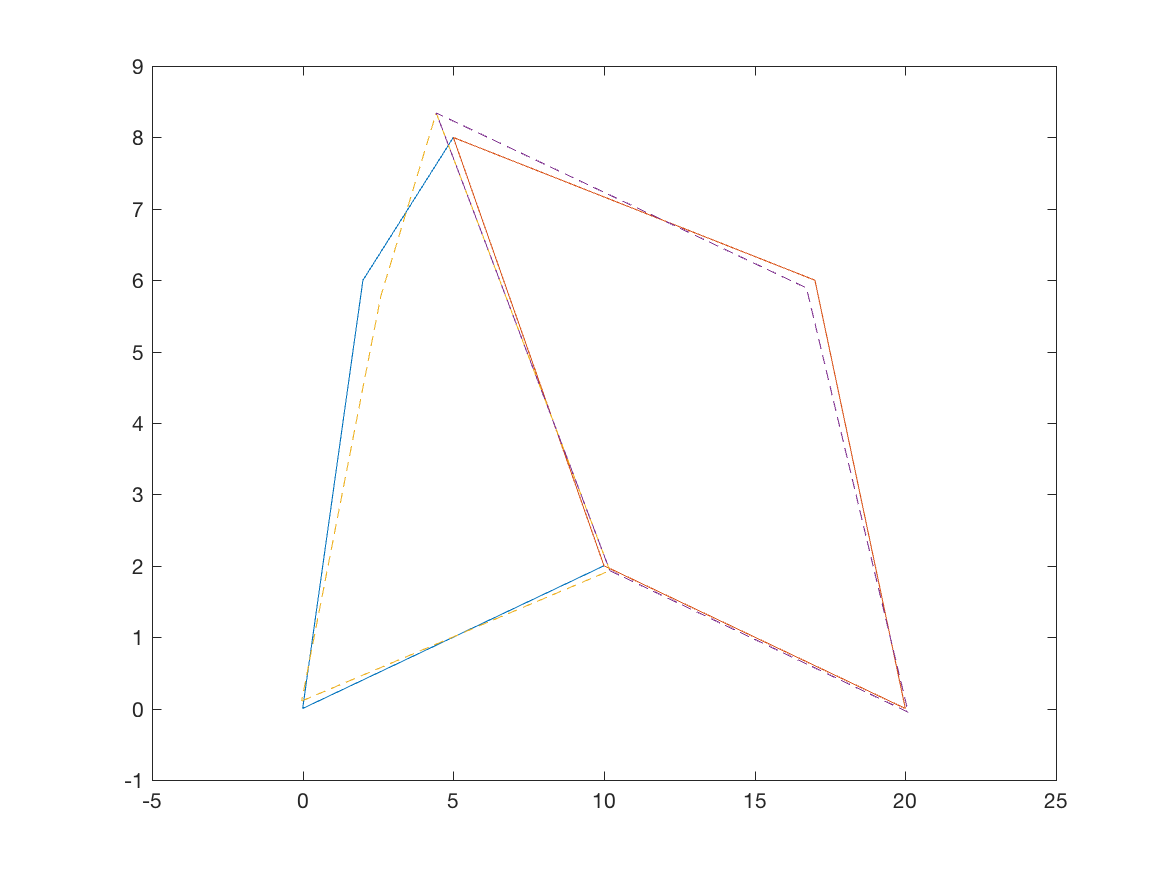
\includegraphics[width=.5\linewidth]{eigenvectors/eigenvector_4_fullint.png} 
    \caption{Eigenvalue 4} 
    \vspace{4ex}
  \end{minipage} 
\end{figure}

\begin{figure}[H] 
  \label{fig2} 
  \begin{minipage}[b]{0.5\linewidth}
    \centering
    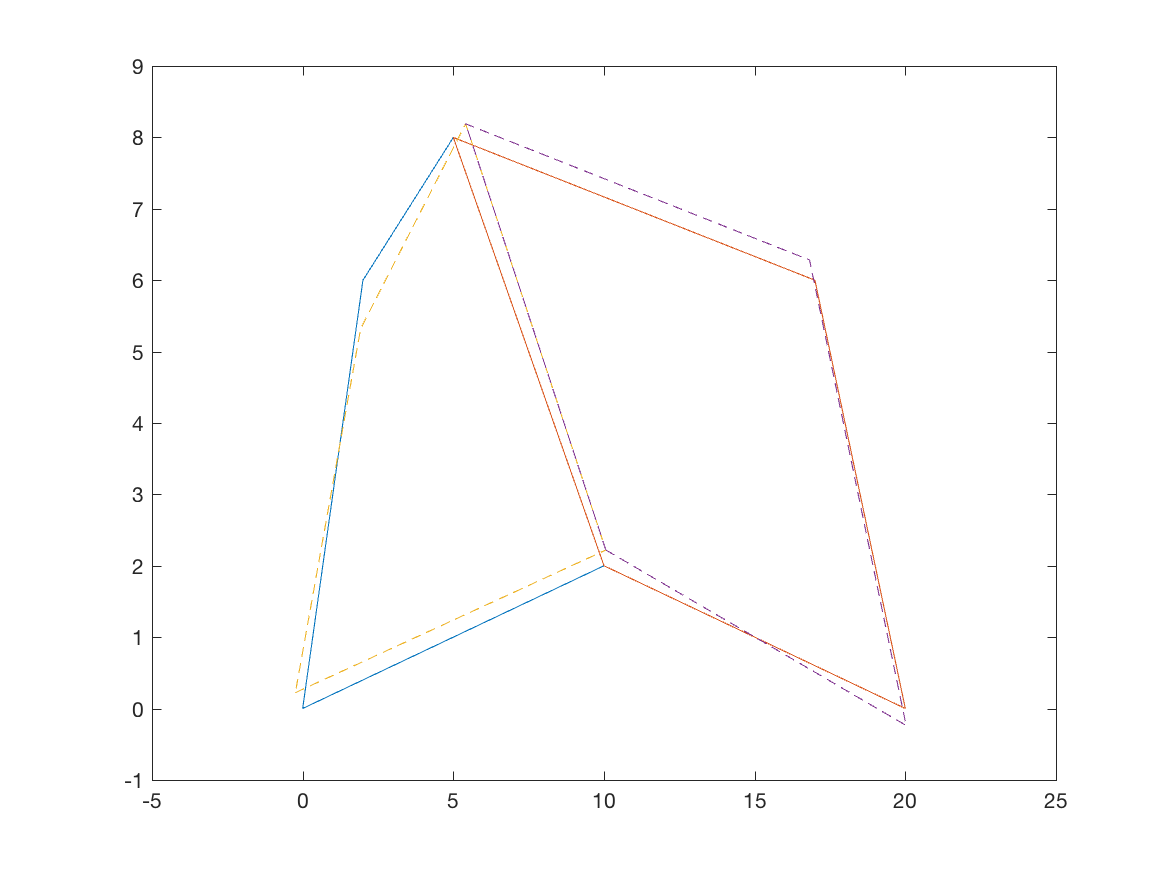
\includegraphics[width=.5\linewidth]{eigenvectors/eigenvector_5_fullint.png} 
    \caption{Eigenvalue 5} 
    \vspace{4ex}
  \end{minipage}%%
  \begin{minipage}[b]{0.5\linewidth}
    \centering
    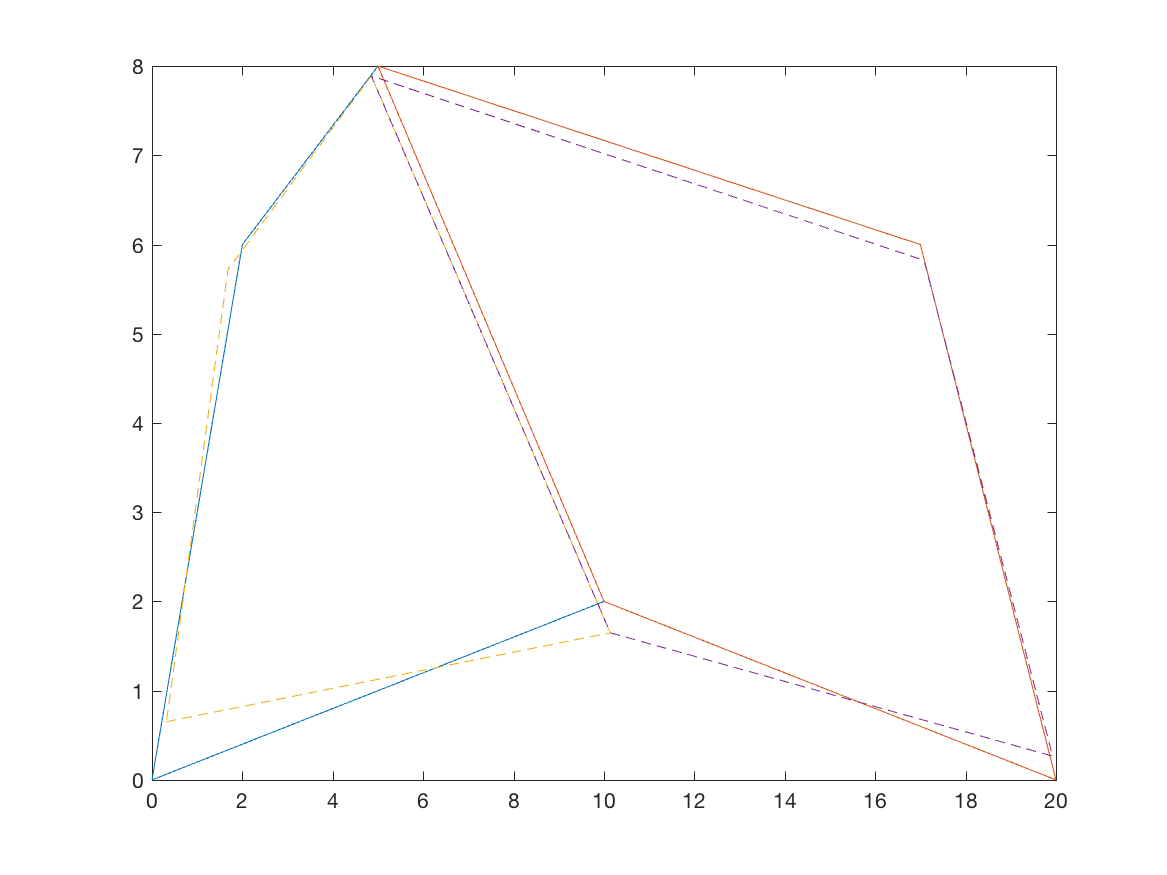
\includegraphics[width=.5\linewidth]{eigenvectors/eigenvector_6_fullint.png} 
    \caption{Eigenvalue 6} 
    \vspace{4ex}
  \end{minipage} 
  \begin{minipage}[b]{0.5\linewidth}
    \centering
    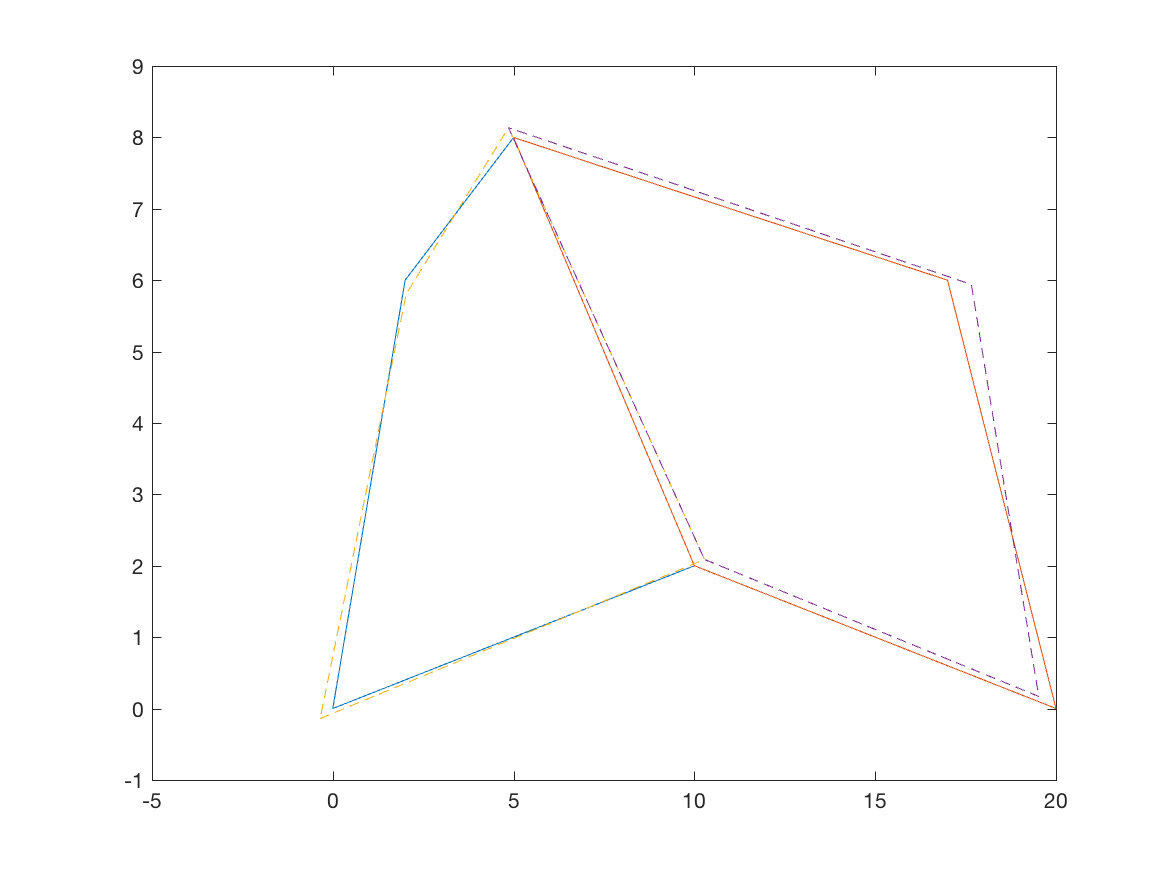
\includegraphics[width=.5\linewidth]{eigenvectors/eigenvector_7_fullint.png} 
    \caption{Eigenvalue 7} 
    \vspace{4ex}
  \end{minipage}%% 
  \begin{minipage}[b]{0.5\linewidth}
    \centering
    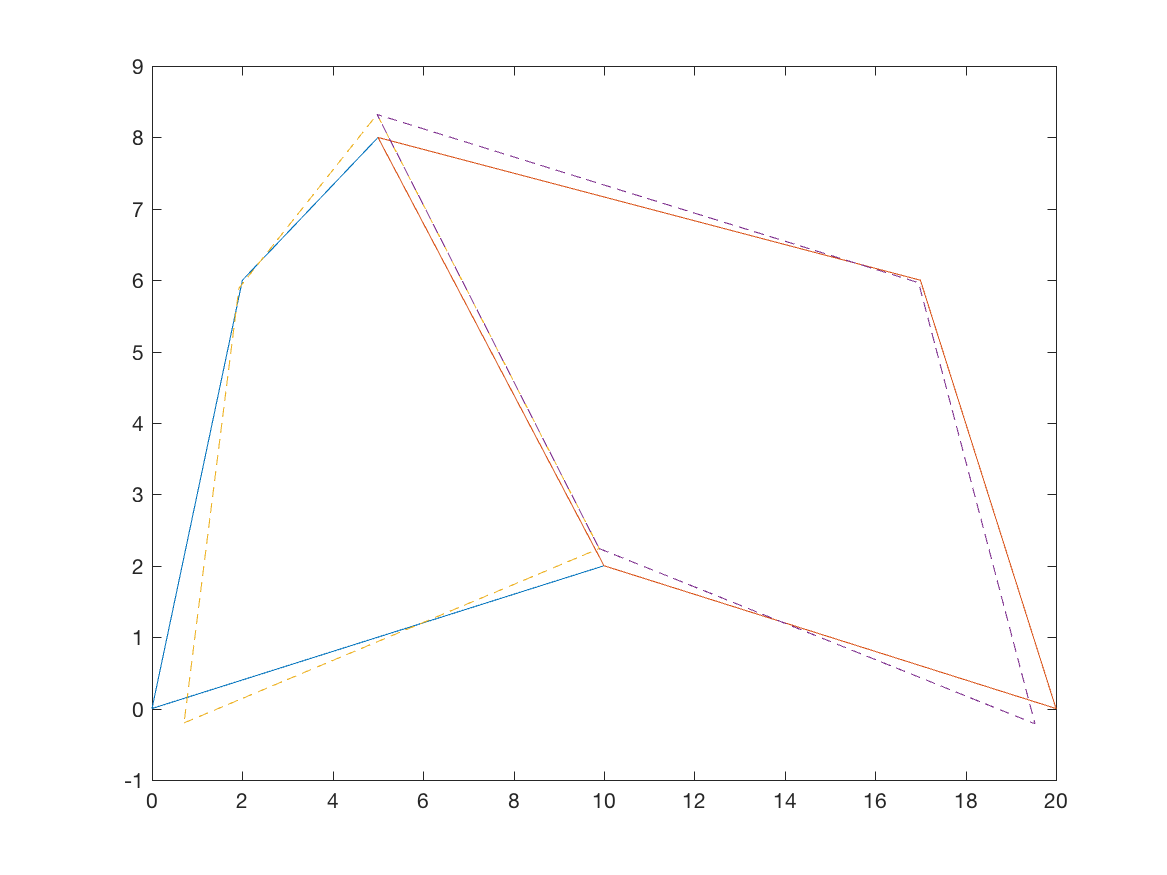
\includegraphics[width=.5\linewidth]{eigenvectors/eigenvector_8_fullint.png} 
    \caption{Eigenvalue 8} 
    \vspace{4ex}
  \end{minipage} 
\end{figure}

\begin{figure}[H] 
  \label{fig3} 
  \begin{minipage}[b]{0.5\linewidth}
    \centering
    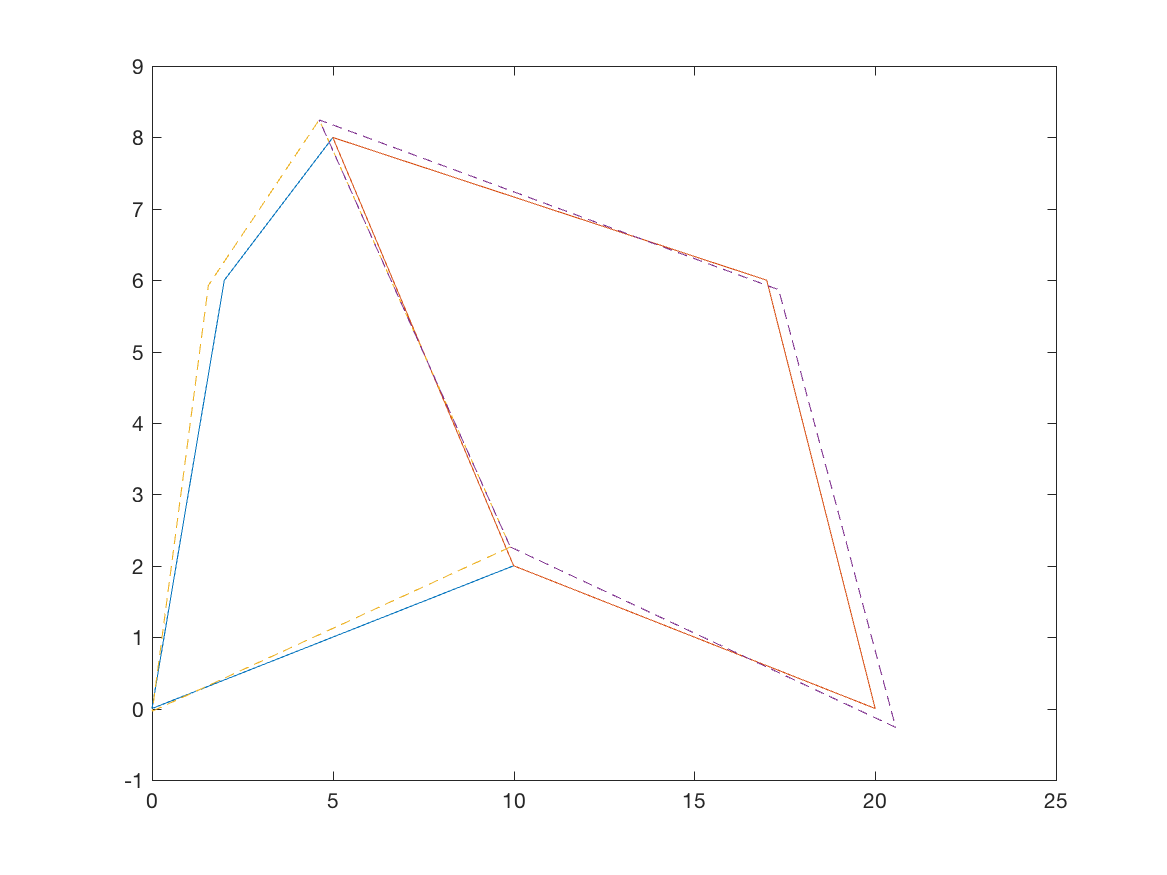
\includegraphics[width=.5\linewidth]{eigenvectors/eigenvector_9_fullint.png} 
    \caption{Eigenvalue 9} 
    \vspace{4ex}
  \end{minipage}%%
  \begin{minipage}[b]{0.5\linewidth}
    \centering
    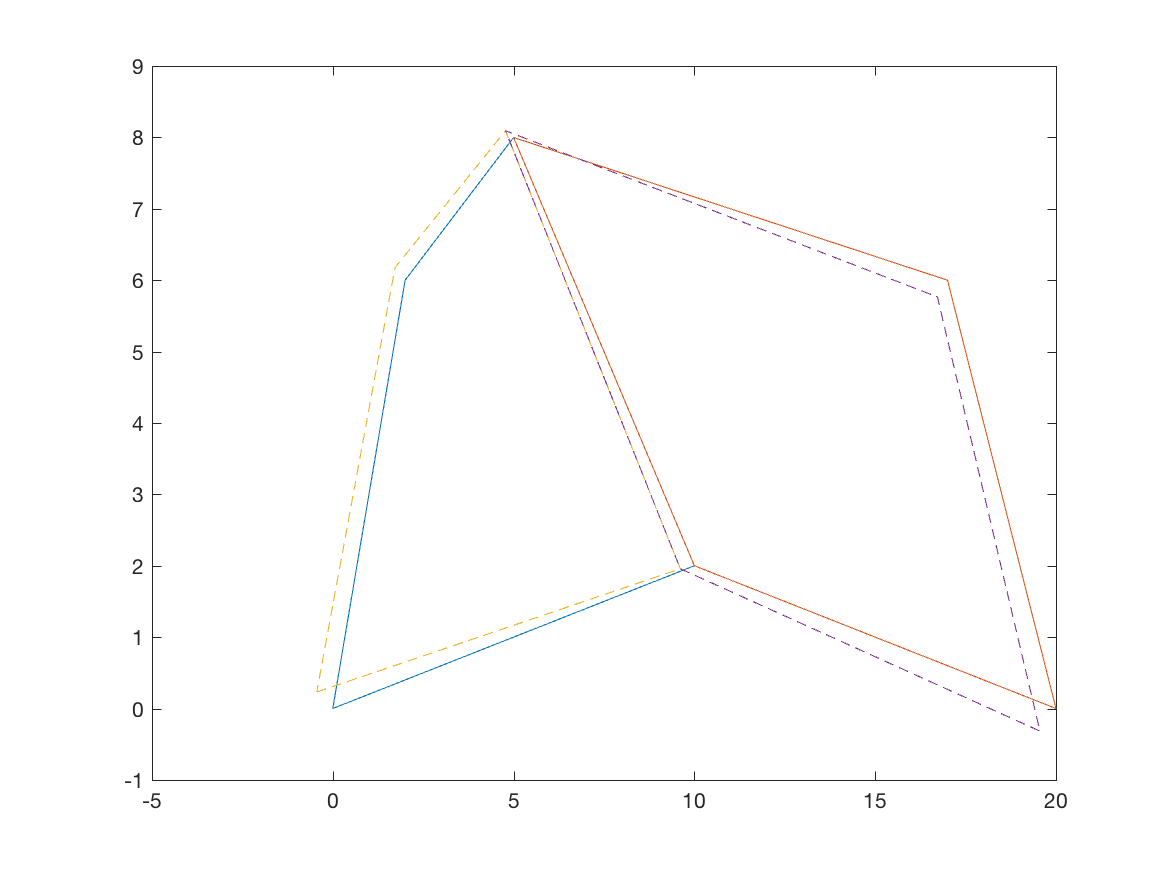
\includegraphics[width=.5\linewidth]{eigenvectors/eigenvector_10_fullint.png} 
    \caption{Eigenvalue 10} 
    \vspace{4ex}
  \end{minipage} 
  \begin{minipage}[b]{0.5\linewidth}
    \centering
    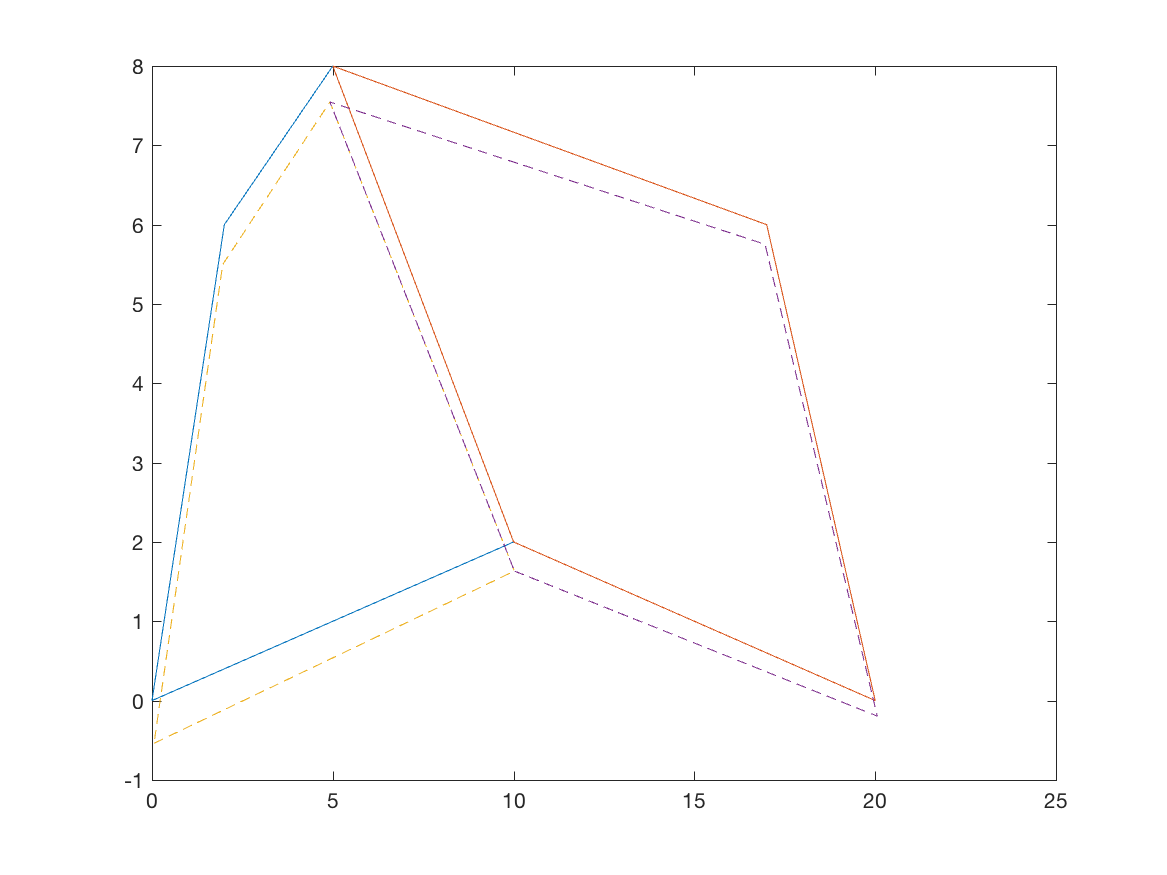
\includegraphics[width=.5\linewidth]{eigenvectors/eigenvector_11_fullint.png} 
    \caption{Eigenvalue 11} 
    \vspace{4ex}
  \end{minipage}%% 
  \begin{minipage}[b]{0.5\linewidth}
    \centering
    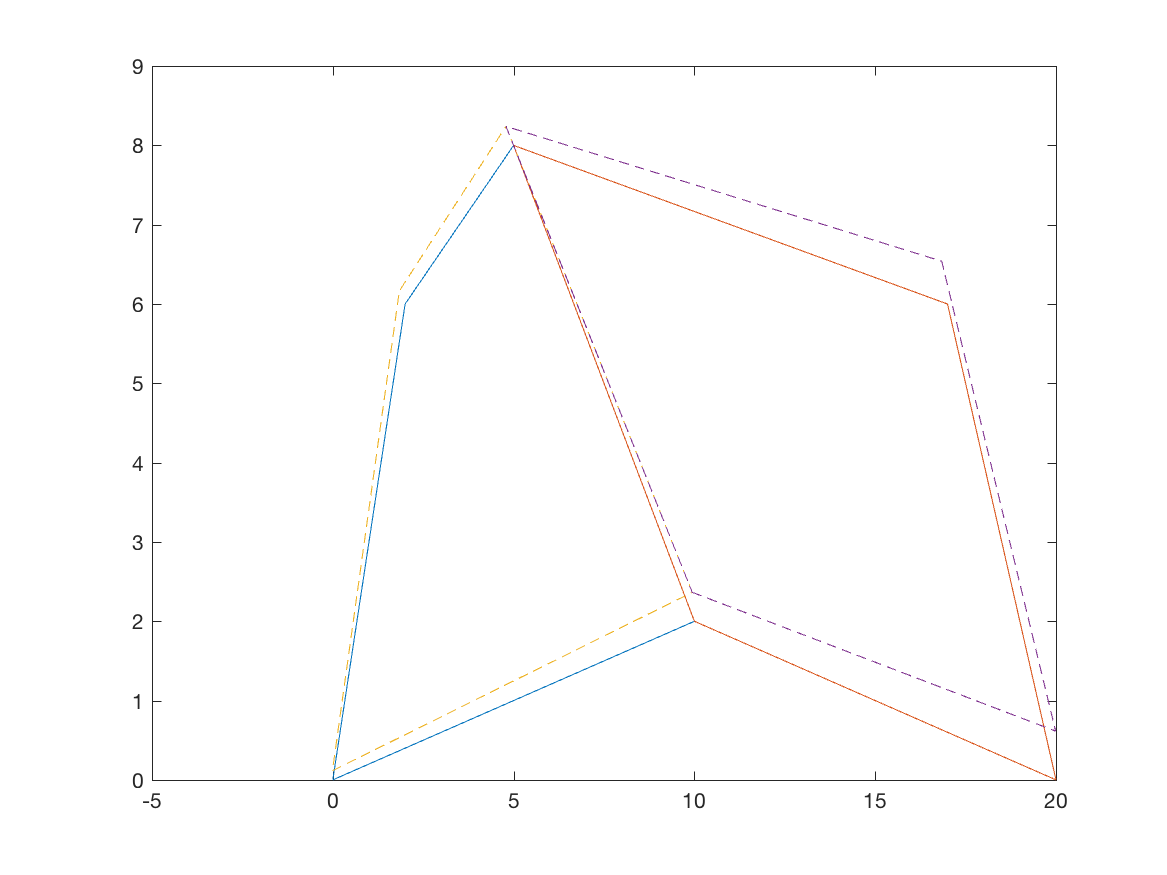
\includegraphics[width=.5\linewidth]{eigenvectors/eigenvector_12_fullint.png} 
    \caption{Eigenvalue 12} 
    \vspace{4ex}
  \end{minipage} 
\end{figure}

\subsection{Comments}


\begin{figure}[H] 
  \label{fig4} 
  \begin{minipage}[b]{0.5\linewidth}
    \centering
    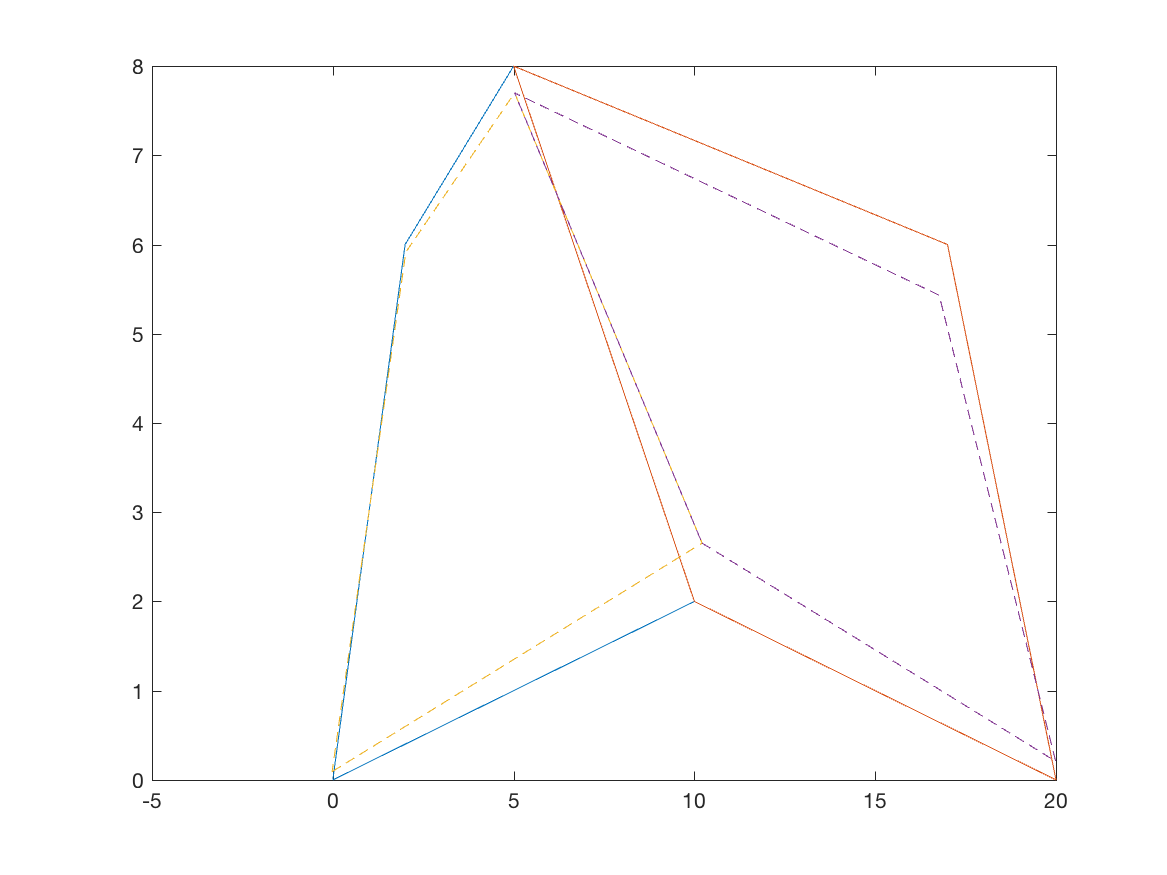
\includegraphics[width=.5\linewidth]{eigenvectors/eigenvector_1_redint.png} 
    \caption{Eigenvalue 1} 
    \vspace{4ex}
  \end{minipage}%%
  \begin{minipage}[b]{0.5\linewidth}
    \centering
    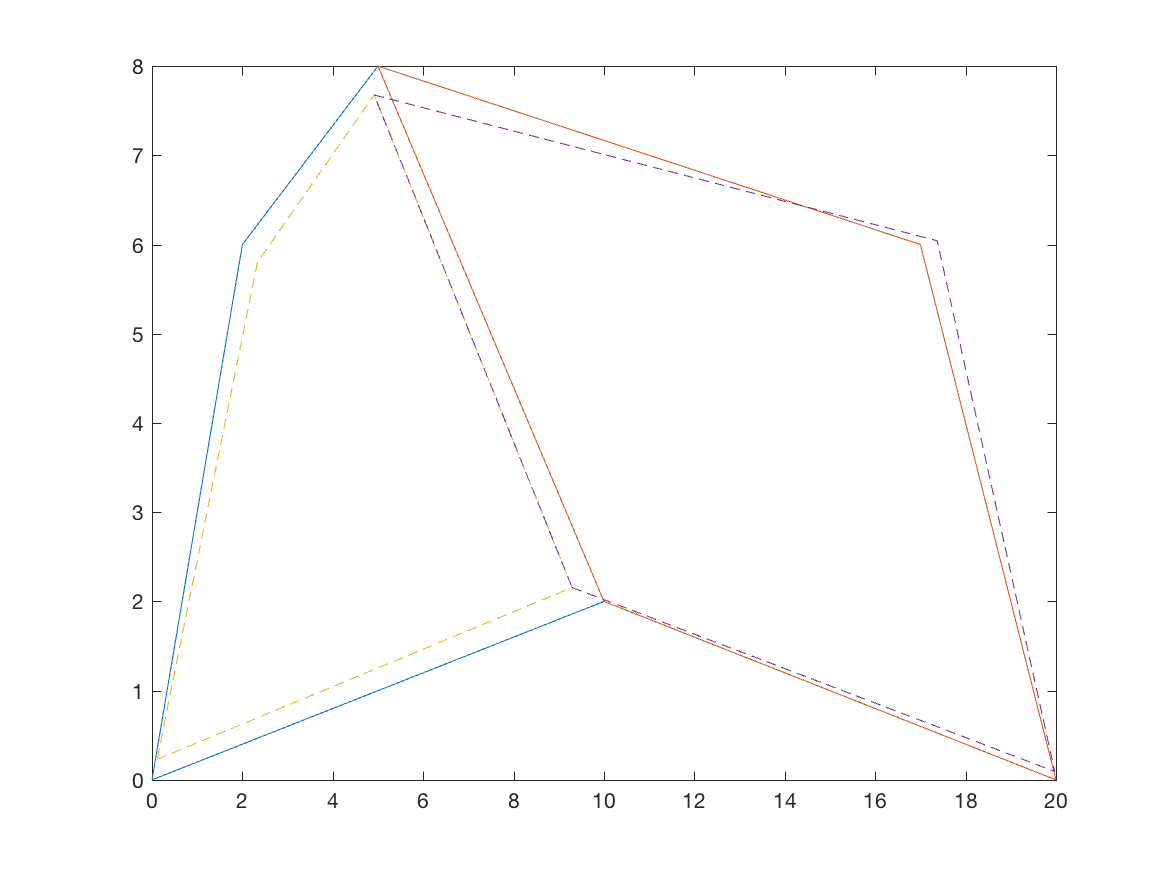
\includegraphics[width=.5\linewidth]{eigenvectors/eigenvector_2_redint.png} 
    \caption{Eigenvalue 2} 
    \vspace{4ex}
  \end{minipage} 
  \begin{minipage}[b]{0.5\linewidth}
    \centering
    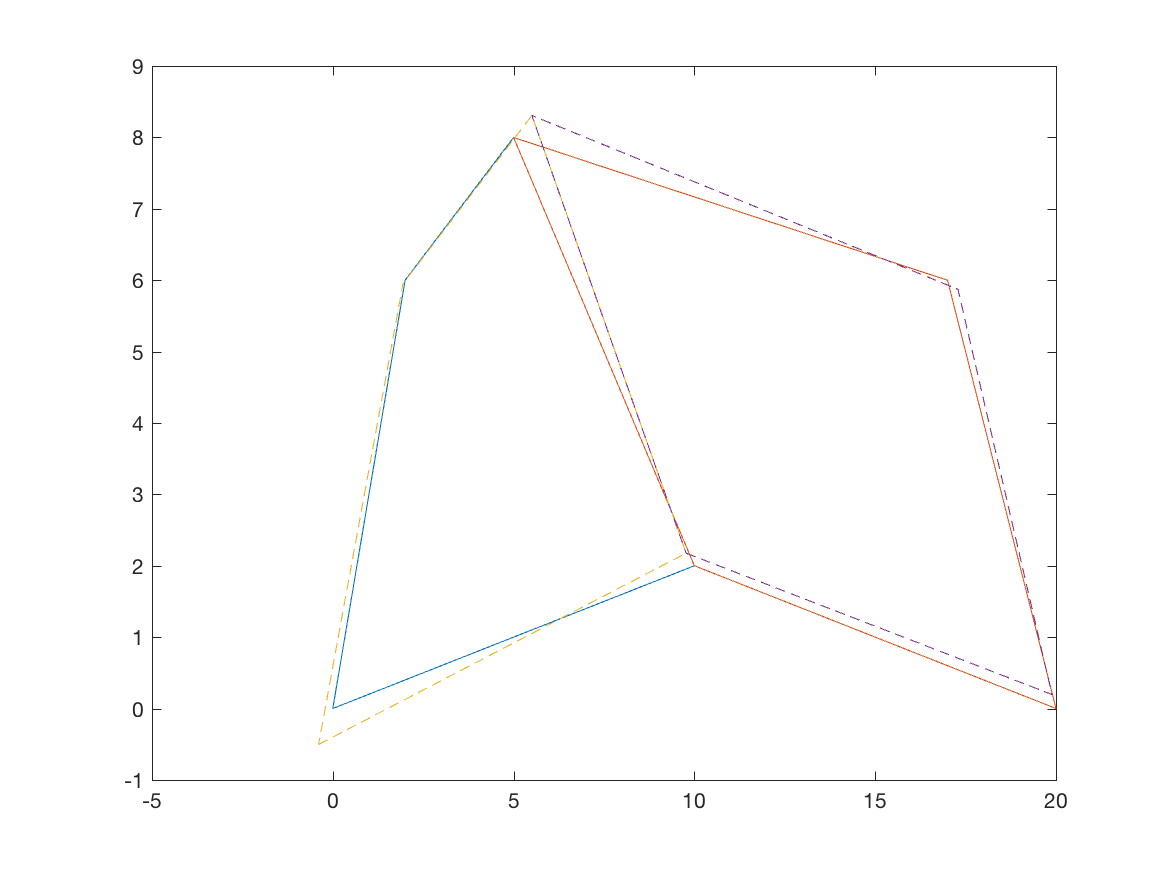
\includegraphics[width=.5\linewidth]{eigenvectors/eigenvector_3_redint.png} 
    \caption{Eigenvalue 3} 
    \vspace{4ex}
  \end{minipage}%% 
  \begin{minipage}[b]{0.5\linewidth}
    \centering
    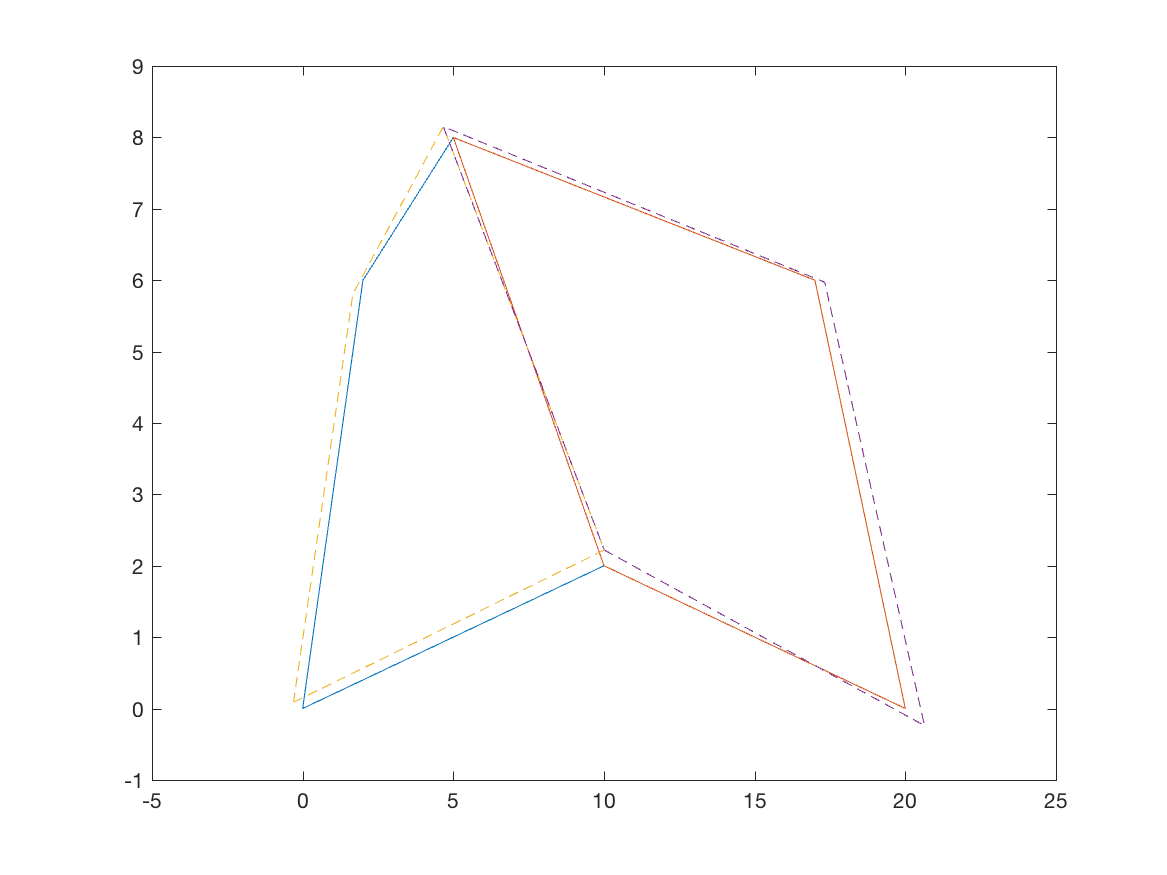
\includegraphics[width=.5\linewidth]{eigenvectors/eigenvector_4_redint.png} 
    \caption{Eigenvalue 4} 
    \vspace{4ex}
  \end{minipage} 
\end{figure}

\begin{figure}[H] 
  \label{fig5} 
  \begin{minipage}[b]{0.5\linewidth}
    \centering
    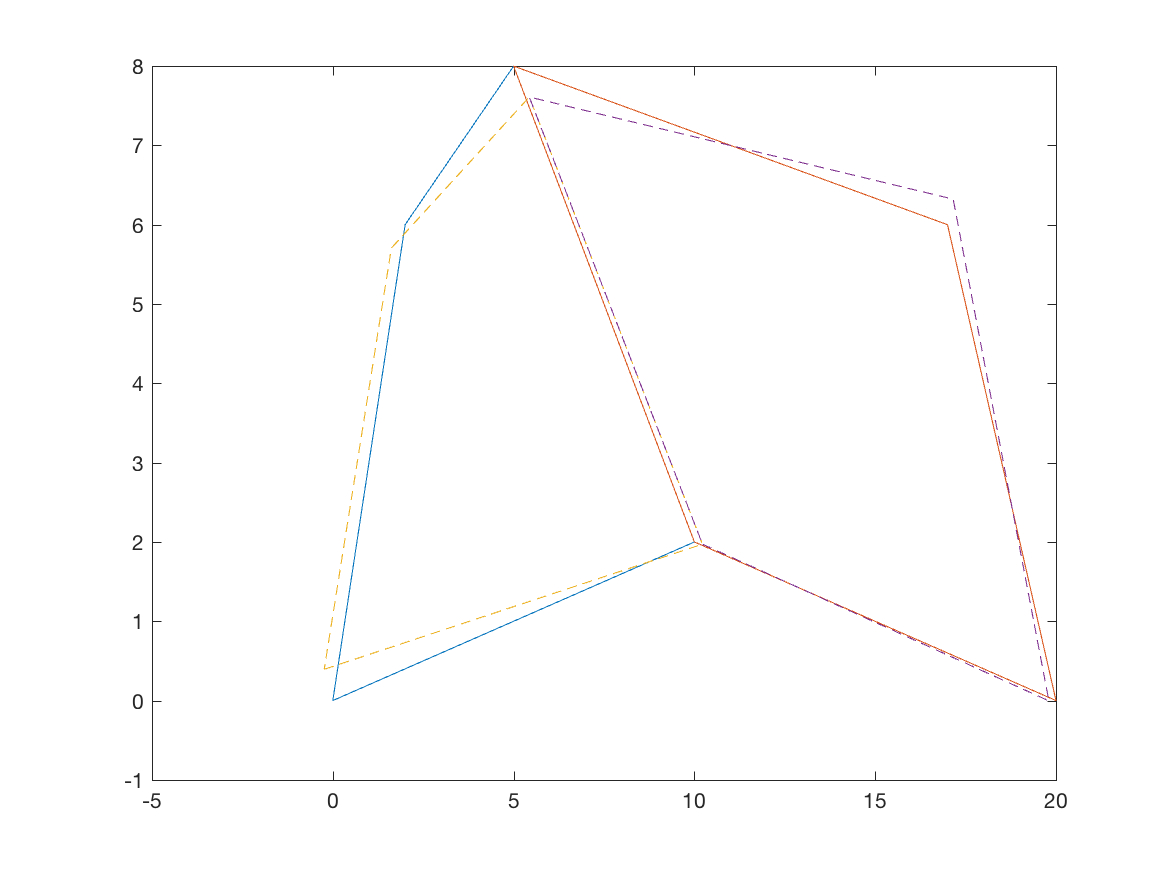
\includegraphics[width=.5\linewidth]{eigenvectors/eigenvector_5_redint.png} 
    \caption{Eigenvalue 5} 
    \vspace{4ex}
  \end{minipage}%%
  \begin{minipage}[b]{0.5\linewidth}
    \centering
    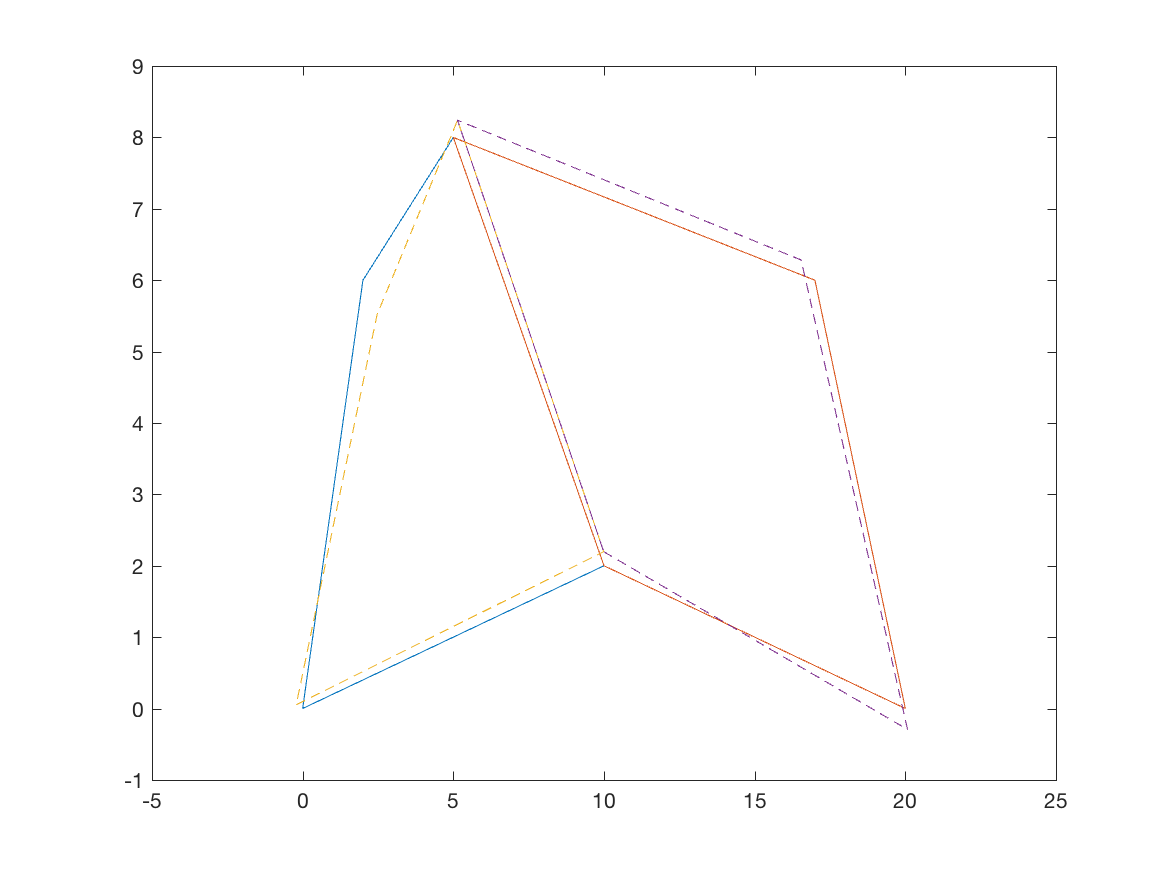
\includegraphics[width=.5\linewidth]{eigenvectors/eigenvector_6_redint.png} 
    \caption{Eigenvalue 6} 
    \vspace{4ex}
  \end{minipage} 
  \begin{minipage}[b]{0.5\linewidth}
    \centering
    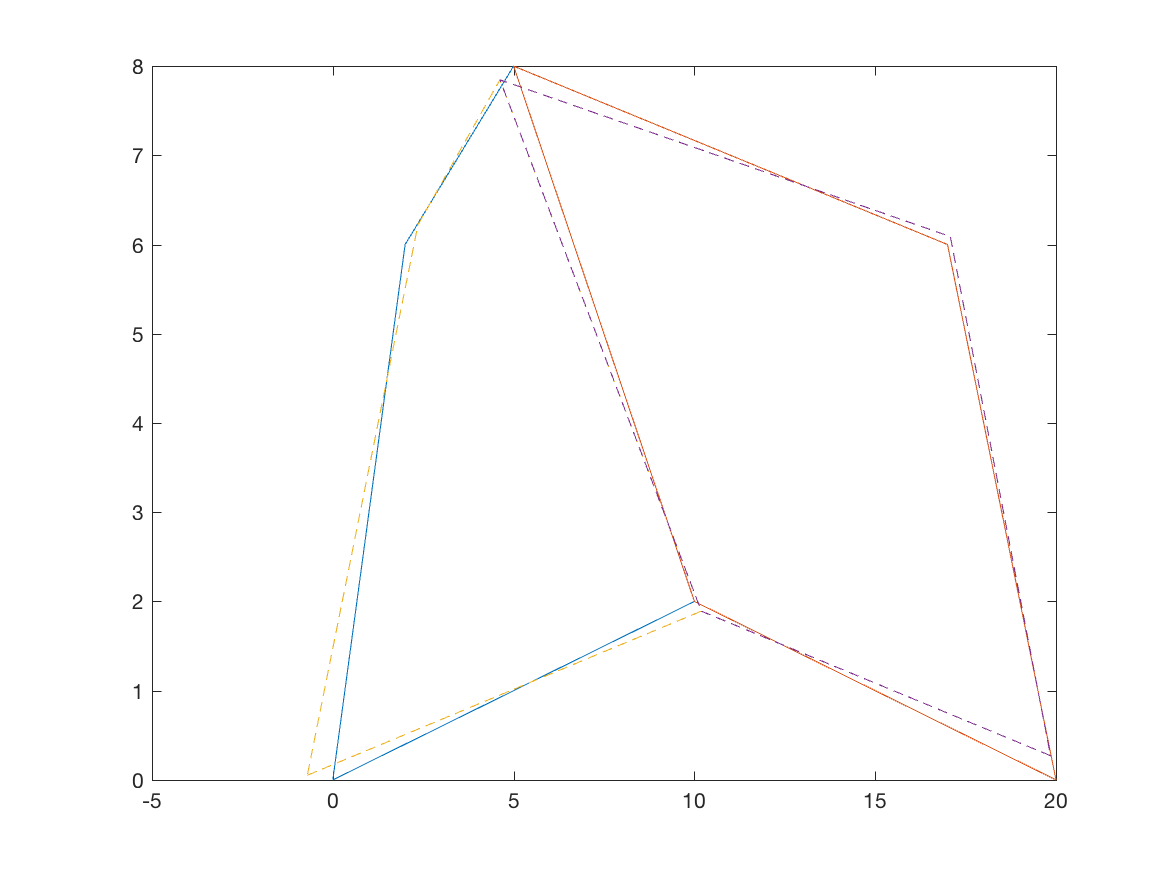
\includegraphics[width=.5\linewidth]{eigenvectors/eigenvector_7_redint.png} 
    \caption{Eigenvalue 7} 
    \vspace{4ex}
  \end{minipage}%% 
  \begin{minipage}[b]{0.5\linewidth}
    \centering
    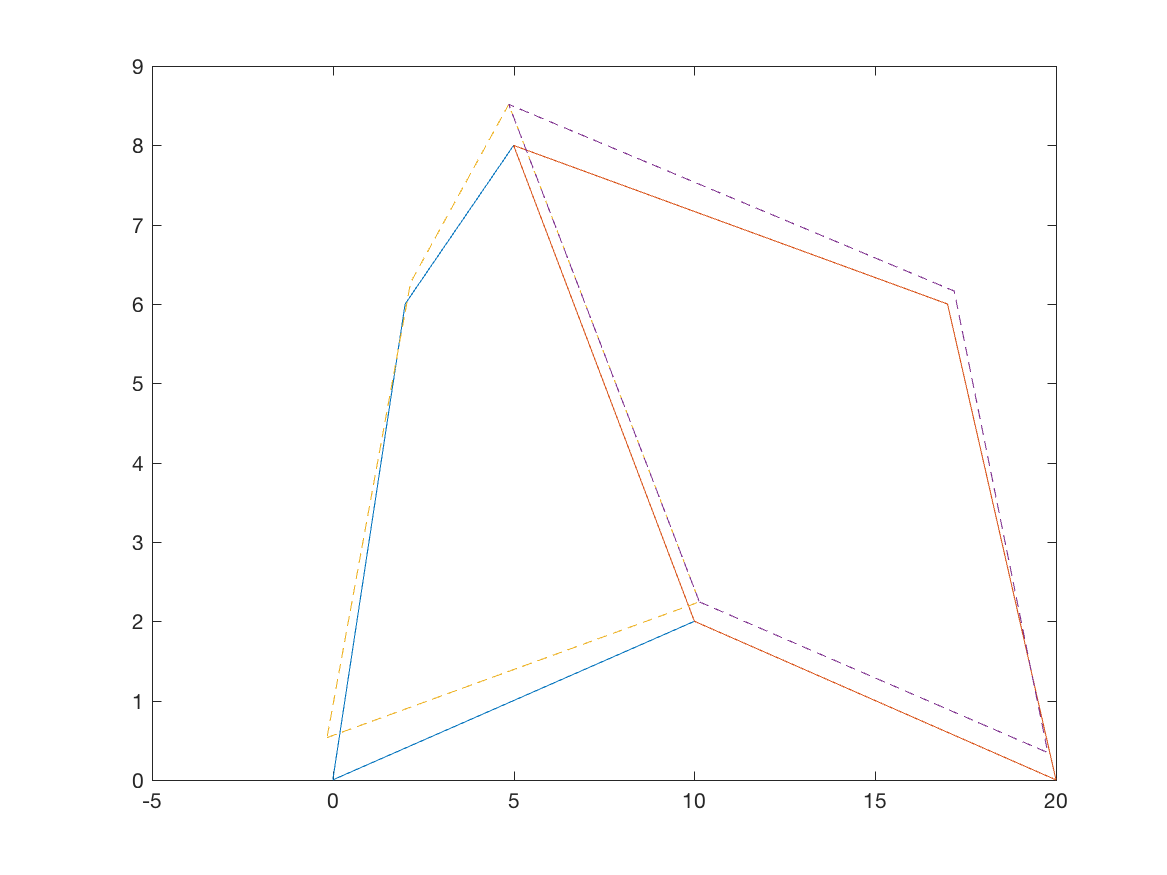
\includegraphics[width=.5\linewidth]{eigenvectors/eigenvector_8_redint.png} 
    \caption{Eigenvalue 8} 
    \vspace{4ex}
  \end{minipage} 
\end{figure}

\begin{figure}[H] 
  \label{fig6} 
  \begin{minipage}[b]{0.5\linewidth}
    \centering
    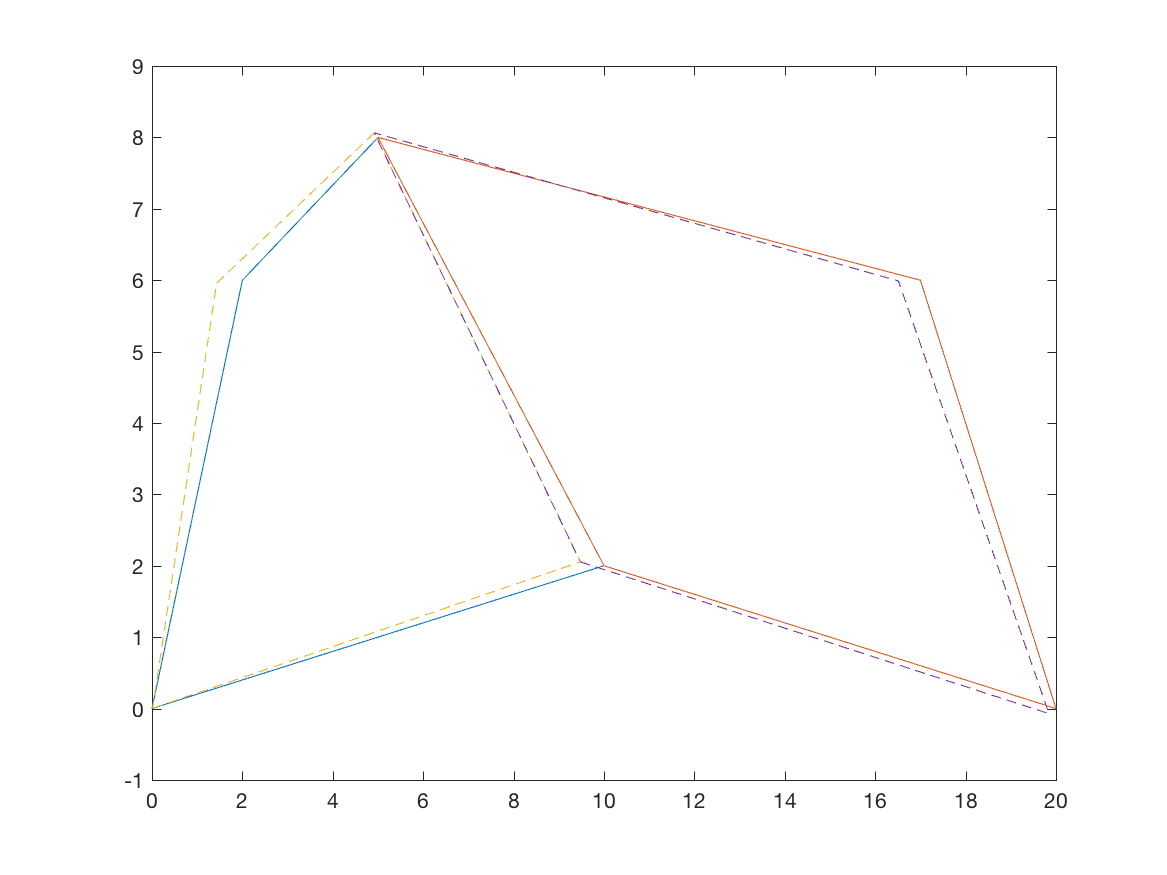
\includegraphics[width=.5\linewidth]{eigenvectors/eigenvector_9_redint.png} 
    \caption{Eigenvalue 9} 
    \vspace{4ex}
  \end{minipage}%%
  \begin{minipage}[b]{0.5\linewidth}
    \centering
    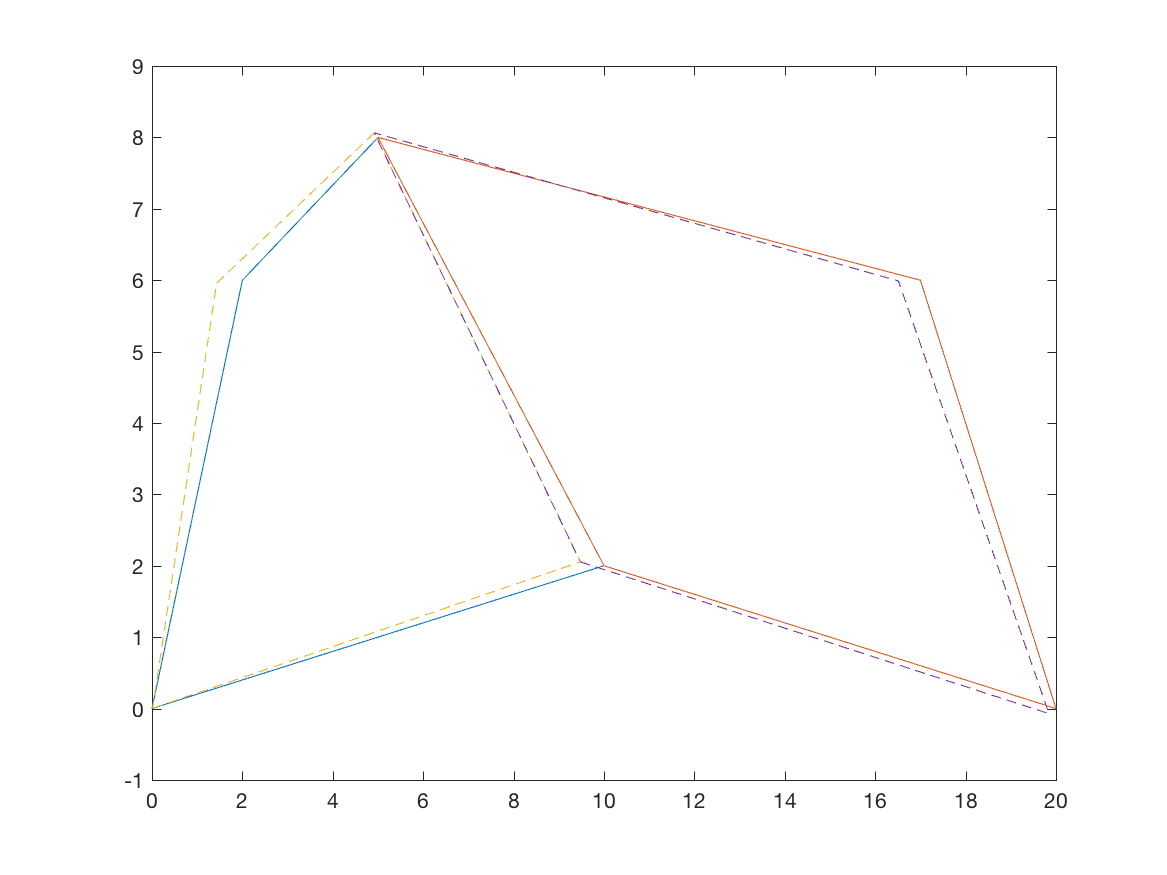
\includegraphics[width=.5\linewidth]{eigenvectors/eigenvector_10_redint.png} 
    \caption{Eigenvalue 10} 
    \vspace{4ex}
  \end{minipage} 
  \begin{minipage}[b]{0.5\linewidth}
    \centering
    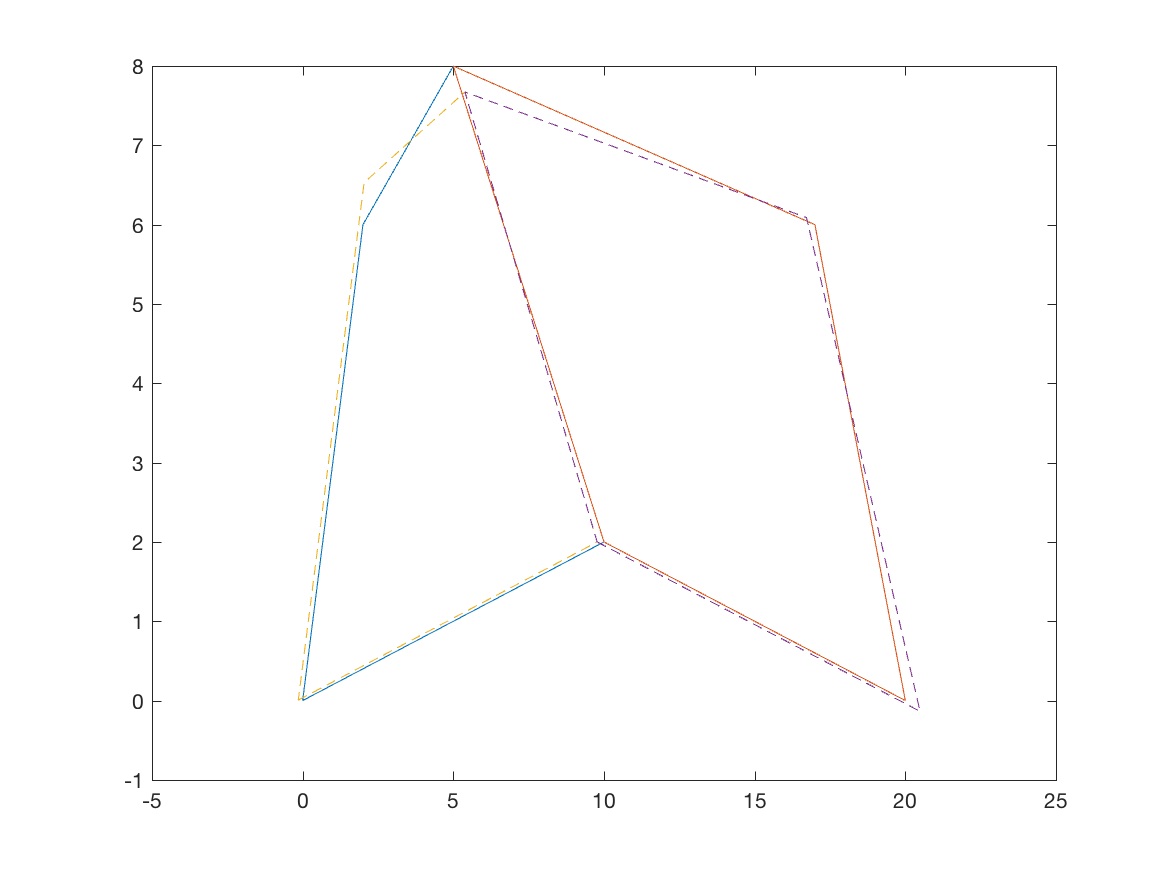
\includegraphics[width=.5\linewidth]{eigenvectors/eigenvector_11_redint.png} 
    \caption{Eigenvalue 11} 
    \vspace{4ex}
  \end{minipage}%% 
  \begin{minipage}[b]{0.5\linewidth}
    \centering
    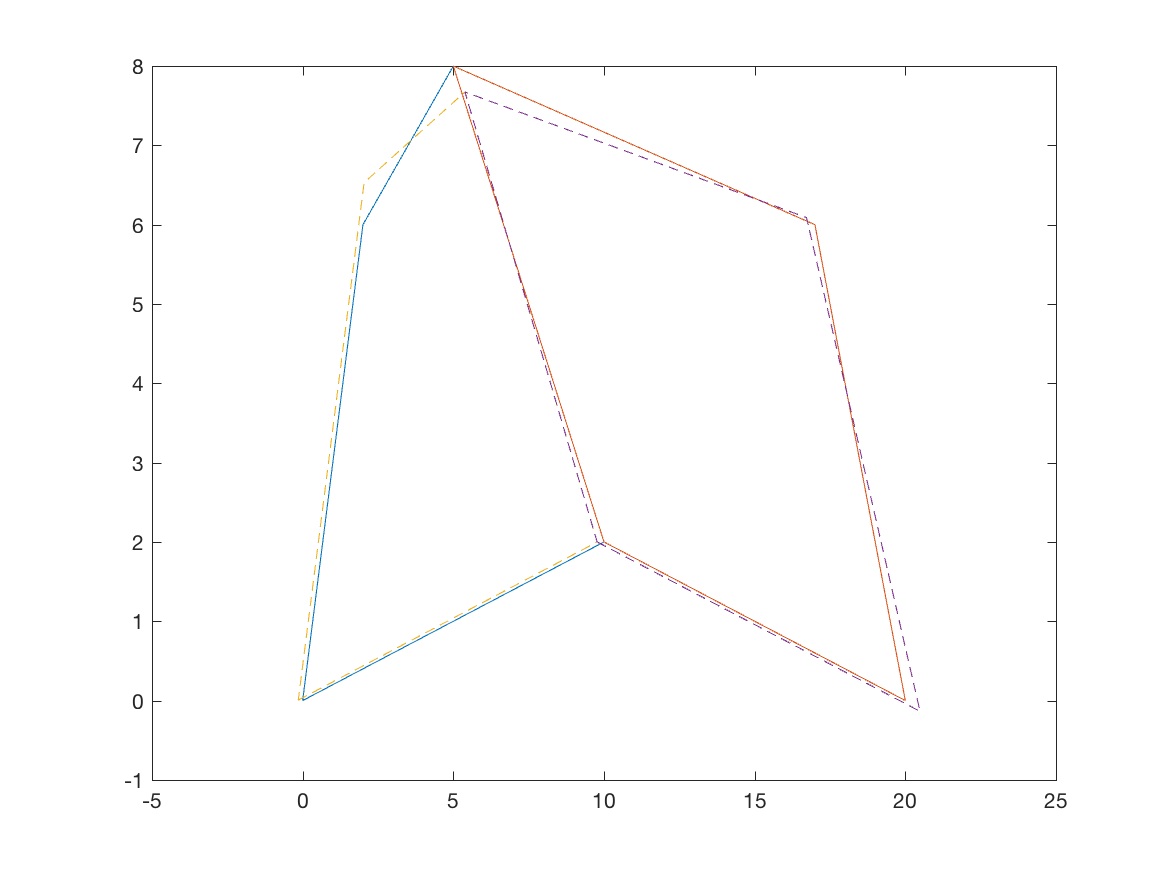
\includegraphics[width=.5\linewidth]{eigenvectors/eigenvector_12_redint.png} 
    \caption{Eigenvalue 12} 
    \vspace{4ex}
  \end{minipage} 
\end{figure}



In the initial case of full integration we had a total of 3 zero eigenvalues (rotation, translation) and for reduced integration we had 6 zero eigenvalues.














\end{document}  